\documentclass[11pt]{standalone}

\usepackage{ifthen}
\usepackage{tikz} 
\usetikzlibrary{shapes.misc}
\usetikzlibrary{arrows,arrows.meta}
\usetikzlibrary{calc,intersections, patterns, math}

\definecolor{pfeil}{RGB}{168,167,167}
\definecolor{petrol}{RGB}{0, 118, 136}
\definecolor{darkgoldenrod}{RGB}{184, 134, 11}
\colorlet{petrol-lighter}{petrol!40}
\colorlet{darkgoldenrod-lighter}{darkgoldenrod!40}

\begin{document}

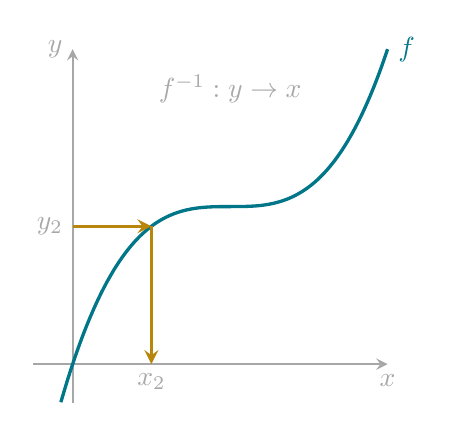
\begin{tikzpicture}[pfeil]

    % \draw[thick, fill=petrol!20, draw=petrol-lighter, rounded corners=2ex, opacity=0.5] (0,0) rectangle ++ (1.5,3.5);
    % \draw[thick, fill=darkgoldenrod!20, draw=darkgoldenrod-lighter, rounded corners=2ex, opacity=0.5] (5,0) rectangle ++ (1.5,3.5);

    \draw[thick, -stealth] (-0.5,0) -- (4,0) node[below]{$x$};
				\draw[thick, -stealth] (0,-0.5) -- (0,4) node[left]{$y$};
				\draw[very thick,domain=-0.15:4, smooth, samples=50, petrol] plot(\x,{0.25*(\x-2)^3+2}) node[right] {$f$};
				\node[left] at (0,1.75) {$y_2$};
				\draw[very thick, darkgoldenrod, stealth-] (1,1.75) -- (0,1.75);
				\draw[very thick, darkgoldenrod, stealth-] (1,0) -- (1,1.75);
				\node[below] at (1,0) {$x_2$};
				\node at (2,3.5) {$f^{-1} : y \rightarrow x$};

\end{tikzpicture}

\end{document}
